\section{Primzahlen}\label{Kapitel Primzahlen}
	Natürliche Primzahlen werden definiert durch Zahlen > 1 die nur durch Eins oder sich selbst teilbar sind. Wie im Kapitel Primfaktorzerlegung gezeigt, können alle natürlichen Zahlen mit einer Multiplikation von Primzahlen erzeugt werden. Sie bilden sozusagen die Bausteine aller natürlichen Zahlen. Die Unberechenbarkeit mit der sie auftreten gibt Mathematikern schon seit Jahrtausenden Rätsel auf und ist ein Grundstein unserer heutigen Verschlüsselungsverfahren.
	In anderen Zahlensystemen als den natürlichen Zahlen ist die gewohnte Definition von Primzahlen nicht vollständig/korrekt. Sie sagt nur etwas über die Irreduzibelität eines Elements in einem Integritätsbereich aus. Da in den natürlichen Zahlen aber jedes irreduzibles Element auch prim ist, reicht diese Definition für \myMenge{N} aus.
	Für alle Integritätsbereiche gilt für die Primheit folgende Definition nach \cite{Algorithmische:Zahlentheorie}:
	
	Ein Element \myMathRM{p \in R\setminus(R^* \cup~\{0\})} heißt prim oder Primelement, wenn für alle \myMathRM{a, b \in R\setminus\{0\}} gilt:	
	\begin{displaymath}
		p~|~ab \Longrightarrow p~|~a~oder~p~|~b.
	\end{displaymath}
		
	Mit Hilfe der Primzahlen kann der Restklassenring \myMenge{Z}/m\myMenge{Z} spezialisiert werden. Ist m eine Primzahl p, so ist \myMenge{Z}/p\myMenge{Z} ein Körper und wird auch \myMenge{F}\myTiefstellen{p} bzw. \myMenge{GF}\myTiefstellen{p} bezeichnet.
	
	Neben den normalen Primzahlen gibt es weitere sogenannte Pseudoprimzahlen. Diese Primzahlen verhalten sich bezogen auf einen Algorithmus genauso wie echte Primzahlen, sie sind jedoch zusammengesetzt. Ein Beispiel für solche Zahlen sind Carmichaelzahlen die in einem späteren Kapitel thematisiert sind.

	Leider gibt es keine bekannten effizienten Verfahren um Primzahlen zu generieren. Dennoch kann man Primzahlen recht einfach raten. Grundsätzlich ist es möglich eine große Anzahl von Zahlen auszuschließen. Man denke an: nur ungerade Zahlen, die Teilungsgesetze und die Tatsache, dass alle Primzahlen > 3 in der Form 4k +1 oder 4k +3, k \myin \myMenge{N} vorliegen. Alle geratenen Zahlen müssen jedoch einem Primzahltest (vgl. Kapitel \ref{Effiziente Primzahltests}) zur Verifizierung unterzogen werden. In \cite{Algebraische:und:zahlentheoretische:Grundlagen:fuer:die:Informatik} ist beschrieben wie ein Generierungsprozess erfolgen kann.

	\subsection{Primfaktorzerlegung}
	Jede natürliche Zahl größer als Eins kann als Produkt von Primzahlen geschrieben werden. Dieser zentrale Satz wird als Fundamentalsatz der Zahlentheorie bezeichnet und kann auf jeden euklidischen Ring R angewendet werden. Eine Primfaktorzerlegung wird mit x \myin R, u \myin R*, \myMathRM{e_1, e_2, ..., e_m} \myin \myMenge{N} wie folgt definiert:	
	\begin{displaymath}
		x = u \cdot p^{e_1}_1 \cdot p^{e_2}_2 \cdot . . . \cdot p^{e_m}_m,
	\end{displaymath}
	wobei  \myMathRM{p_1 < p_2 < ... < p_m} Primelemente sind.
	
	Neben der Existenz einer solchen Primfaktorzerlegung ist auch die Eindeutigkeit, die durch das Vergleichszeichen \grqq kleiner als\grqq ~implizit angegeben ist, von entscheidender Bedeutung. In \cite{Einfuehrung:in:Algebra:und:Zahlentheorie} und \cite{Algorithmische:Zahlentheorie} wird die Existenz und Eindeutigkeit bewiesen.

	Die meisten kryptographischen Algorithmen bauen auf die ineffiziente Berechnung der Primfaktoren. Es ist zwar einfach zwei Primzahlen miteinander zu multiplizieren, aber es ist schwer aus der multiplizierten Zahl die beiden Primfaktoren zurückzugewinnen. Kennt man jedoch eine der beiden Primzahlen, so berechnet sich die zweite durch einfache Division. Zur Verschlüsselung ergibt sich damit die Idee einer sogenannten Falltür-Funktion, die die Primfaktoren mit Hilfe eines geheimen Hinweises schnell berechnen kann.
		
	\subsection{Satz von Euler und Kleiner Satz von Fermat}
	Die Vermutung vom kleinen Satz von Fermat wurde von Fermat im 17. Jahrhundert aufgestellt und von Euler bewiesen. Euler konnte zudem zeigen, dass der kleine Satz von Fermat nur ein Spezialfall für Primzahlen darstellt. Der Satz von Euler lautet:
	
	Sei m \myGroesserGleich 2 \myin \myMenge{N}. Dann gilt für jede zu m teilerfremde Zahl a \myin \myMenge{N}
	\begin{displaymath}
		a^{\varphi(m)} \equiv~1~mod~m.
	\end{displaymath}
	Denn wie in \cite{Algorithmische:Zahlentheorie} anhand der Gruppentheorie bewiesen, ist
	\begin{displaymath}
		a^{Ord(G)} = a^{|G|} = e,
	\end{displaymath}
	wobei G eine endliche Gruppe ist, a \myin G und e das Einselement (neutrales Element einer multiplikativen Gruppe). Da das Einselement in \myMenge{N} 1 ist, folgt: Kongruenz 1 modulo m. 
	
	Des weiteren ergibt sich mit \myMathRM{\varphi(p) = Card((\mathbb{Z}/p\mathbb{Z})^*)} =
	\myMathRM{ |\mathbb{F}^*_p| = p-1} sofort der kleine Satz von Fermat:
	\begin{displaymath}
		a^{p-1} \equiv~1~mod~p
	\end{displaymath}
		
	Mit dem Satz von Euler und Fermat kann nun ein erster primitiver Primzahltest definiert werden.  
	Für ein beliebiges 	a \myin \myMenge{N} mit 1 < a < m gilt:
	\begin{displaymath}
		a^{m-1} \not\equiv 1~mod~m \Longrightarrow nicht~prim
	\end{displaymath}
	Leider ist der fermatsche Primzahltest nur ein negativ Test, der eindeutig zeigen kann, dass eine Zahl nicht prim ist. Wenn der Test einer Zahl kongruent 1 modulo m ergibt, muss m also nicht prim sein. Eine Zahl, die für den Test prim ist, ist entweder eine echte Primzahl oder eine Pseudoprimzahl m zur Basis a.\cite{Elementare:Zahlentheorie}
		
	\subsection{Carmichaelzahlen}
	Da Pseudoprimzahlen die Primalität immer zu einer Basis aufweisen, liegt der Versuch nahe andere Basen zu suchen, für die der fermatsche Test nachweisen kann, dass die vermeintliche Primzahl gar keine ist. Dies ist der Grundbaustein für probabilistische Primzahltests. Dennoch gibt es Zahlen für die der fermatsche Test bei allen teilerfremden Basen kongruent eins Äquivalenz feststellt. Diese starken fermatschen Pseudoprimzahlen heißen Carmichaelzahlen.
	
	Carmichaelzahlen werden nach \cite{Algebraische:und:zahlentheoretische:Grundlagen:fuer:die:Informatik} so definiert:
	
	Eine zusammengesetzte Zahl m \myin \myMenge{N}, m \myMathRM{\geq} 3, heißt Carmichaelzahl genau dann, wenn für alle Basen a mit ggT(m, a) = 1 gilt: 
	\begin{displaymath}
		a^{m-1} \equiv 1~mod~m
	\end{displaymath}
	Die weiteren zwei folgenden Eigenschaften seien zudem genannt, da sie für den probabilistischen Primzahltest von Miller und Rabin von entscheidender Bedeutung sind.
	
	Eine zusammengesetzte Zahl m \myMathRM{\geq} 3 \myin N ist eine Carmichaelzahl, wenn m keine mehrfachen gleichen Primfaktoren enthält und jeder Primfaktor p | m auch 
	\begin{displaymath}
		p-1~|~m-1
	\end{displaymath}
	gilt.	
	
	\subsection{Sieb des Eratosthenes}
	Das Sieb des Eratosthenes ist eines der ältesten bekannten Verfahren um Primzahlen zu erhalten. Es berechnet für ein gegebenes n \myin \myMenge{N} alle Primzahlen p \myin \myMenge{N}, für die gilt 1 < p < n. Der Algorithmus iteriert dazu über alle nicht gestrichenen Zahlen von 1 bis \myMathRM{\sqrt{n}}. Als erstes wird die Zahl Zwei genommen, sie ist nicht gestrichen und somit eine Primzahl. Dann werden alle Vielfache von Zwei gestrichen (die geraden Zahlen). Anschließend sucht der Algorithmus die nächste nicht gestrichene Zahl. In diesem Fall ist es die Drei und es werden wieder alle Vielfache von drei gestrichen. Das Verfahren wiederholt sich bis die Suche \myMathRM{\sqrt{n}} erreicht hat. Alle nicht gestrichen Zahlen sind die Primzahlen bis n. Die Abbildung \ref{ABBILDUNG_Primzahlen_100} illustriert die Primzahlen bis 100.
	Wie in \cite{Algebraische:und:zahlentheoretische:Grundlagen:fuer:die:Informatik} gezeigt, hat das Sieb des Eratosthenes eine subexponentielle Laufzeit, da die Laufzeit von der Länge der Eingabe abhängt. Aus diesem Grund eignet es sich nicht für einen praktischen Primzahltest.
	\begin{figure}
		\centering
		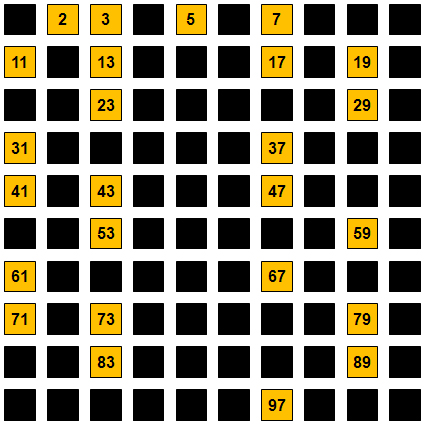
\epsfig{file=includes/images/primzahlen100.jpg, height=3in, width=3in}
		\caption{Primzahlen bis 100 Quelle: \cite{Mathe:Lexikon:SiebDesEratosthenes}}
		\label{ABBILDUNG_Primzahlen_100}
	\end{figure}
	
	\subsection{Effiziente Primzahltests} \label{Effiziente Primzahltests}
		Die in diesem Kapitel vorgestellten Algorithmen zum Erkennen von Primzahlen sind effiziente Algorithmen im Sinne der Komplexitätsklasse P und im Gegensatz zum fermatschen Test nicht anfällig für starke Pseudoprimzahlen. Dennoch unterscheiden sich die beiden vorgestellten Verfahren deutlich voneinander. Neben der Funktionsweise wird auch die Laufzeit gegenübergestellt.
		
		\subsubsection{Miller-Rabin-Test}
		 Der Miller-Rabin-Test ist ein probabilistischer Primzahltest und gehört zu den Montecarlo- Algorithmen. Im Gegensatz zum fermatschen Primzahltest ist der Miller-Rabin-Test nicht so anfällig für Carmichaelzahlen, denn es können immer Basen gefunden werden die die Carmichaelzahlen entlarven. Dieser Test wird am häufigsten in Primzahlgeneratoren eingesetzt und hat damit die größte praktische Relevanz. Nach der Vorstellung des Tests werden die Unterschiede zum fermatschen Test herausgearbeitet.
		 
		 Der Test lautet wie folgt:
		 
		 Wenn m \myin \myMenge{N} > 9  eine ungerade Zahl und \myMathRM{m - 1 = 2^tn} mit ungeradem n ist, dann gilt für jede teilerfremde Zahl a \myin \myMenge{Z}:
		 
	 	\begin{equation} \label{eq:Miller}
			a^n \equiv 1~mod~m~oder~\exists s \in \{0,..., t - 1\} : a^{2^sn} \equiv -1~mod~m
		\end{equation}
		dann ist m prim oder nicht prim.
		
		Aber wenn m nicht prim ist so gilt außerdem für die Menge A aller zu m teilerfremden a, 0 < a < m die (\ref{eq:Miller}) erfüllen:
	 	\begin{equation}
		 	Card(A) \leq 1/4 \varphi(m)
	 	\end{equation}
	 	Durch diese zusätzliche Aussage kann eine Wahrscheinlichkeit angegeben werden mit der die getestete Zahl prim ist. Wiederholt man den Test t mal ergibt sich somit eine Wahrscheinlichkeit von \myMathRM{1/4^t}. Nach zehn Iterationen ist somit die Wahrscheinlichkeit für eine zusammengesetzte Zahl kleiner als \myMathRM{10^{-6}}.
	 	
	 	Um die Ausdrücke in (\ref{eq:Miller}) zu verstehen müssen folgende Vorüberlegungen gemacht werden.
	 	Jeder Körper \myMathRM{F^*_p} kann nach \cite{Algorithmische:Zahlentheorie} in die zwei Teile (Untergruppen) der Quadrate und nicht Quadrate geteilt werden. Jede dieser Gruppen besteht aus \myMathRM{Card(F^*_p)/2 = (p-1)/2} Elementen. Dies folgt aus der Tatsache das \myMathRM{x^2 \equiv~a~mod~p} in \myMathRM{F^*_p} nur die Lösungen +1 oder -1 hat. Ein Element ist ein Quadrat wenn es gleich dem quadratischen Rest eines \myMathRM{x^2~mod~p} ist.
	 	
	 	Eine weitere Überlegung ergibt sich aus dem umgekehrten Satz des Eulerkriteriums der wie folgt lautet.
	 	Sei \myMathRM{m \geq 3} eine ungerade ganze Zahl, so dass (m - 1)/2 ungerade ist.
	 	Es gilt dann für jede zu m teilerfremde ganze Zahl a
	 	\begin{equation}
		 	a^{(m-1)/2} \equiv~^+_-1~mod~m,
	 	\end{equation}
	 	so dass m eine Primzahl ist.
	 	
	 	Wenn (m - 1)/2 gerade ist kann diese Aussage nicht getroffen werden. Für den Fall das m eine Carmichaelzahl ist, ist auch \myMathRM{m - 1 = 2^{s_i}u_i(p_i - 1)} , da alle Primfaktoren m-1 teilen, wobei \myMathRM{u_i} ungerade ist. Es gilt dann O.B.d.A mit \myMathRM{s_1 \leq s_2 \leq . . . \leq s_r~und~s = s_1}:
 		\begin{displaymath}
	 		a^{(m-1)/2^s} \equiv1 ~fuer~alle~a \in \mathbb{Z}^*_m
 		\end{displaymath}
 		Anschließend müssen wie in \cite{Algorithmische:Zahlentheorie} durchgeführt, mehrere Fallunterscheidungen für gerade und ungerade vielfache von (\myMathRM{a^{(m-1)/2^{s+1}}}) durchgeführt werden. Dabei können die Ergebnisse der Kongruenzen in Teilmengen eingeteilt werden. Die Kardinalität der Mengen gibt dabei die Wahrscheinlichkeit der Zusammengesetzten Zahlen vor.
 		
 		Etwas abstrakter dargestellt zielt der Test darauf ab im Gegensatz zu dem fermatschen Test die Quadratwurzeln der Carmichaelzahlen in dem Primzahlkriterium zu berücksichtigen. Durch diese Erweiterung kommt es nur noch maximal bei einem Viertel der Basen zur Annahme es handle sich um eine Primzahl.
 		
 		Wie in \cite{Algebraische:und:zahlentheoretische:Grundlagen:fuer:die:Informatik} angegeben benötigt der Test, da die Exponentiation effizient berechenbar ist, O(t * (log m)) arithmetische Operationen und O(t * (log m)\myMathRM{^3}) Bit Operationen bezogen auf die Eingabelänge von m. Damit liegt der Test in der polynomialen Laufzeitklasse.
 		
 		Eine interessante Aussage die in \cite{Algorithmische:Zahlentheorie} getroffen wird, ist dass der Miller-Rabin-Test unter Annahme der Riemannschen Vermutung zu einem deterministischen polynomialen Test wird.
 		
 		%TODO Hier Pseudocode


		\subsubsection{AKS-Test}
		Der 2004 von M. Agrawal, N. Kayal und N. Saxena entwickelte AKS-Test ist ein deterministischer in polynomialer Zeit durchführbarer Primzahltest. Bei diesem Test stellt die Rechnung in einem Polynomring (\myMenge{Z}/m)[X] den größten Unterschied zu den bisherigen Tests da. Besonders wertvoll ist hier die notwendige und hinreichende Bedingung für die Primmalität des folgenden Satzes. 
		
		Der Satz lautet in \cite{Algorithmische:Zahlentheorie} wie folgt:
		Sei m > 1 eine natürliche Zahl und a eine zu m teilerfremde ganze
		Zahl. Genau dann ist m prim, wenn
		\begin{displaymath}
			(X + a)^m \equiv X^m + a~mod~m
		\end{displaymath}
		
		Dieser Satz ist natürlich noch nicht schneller als die Probedivision bis \myMathRM{\sqrt{m}}, aber folgende Erweiterungen führen zu einem polynominelle Laufzeitverhalten. Die Idee hinter der Erweiterung ist ein Polynom zu finden das mit getestet 
		wird und dadurch die Laufzeit reduziert. Ein solches Polynom ist \myMathRM{P(x) = x^r - 1}, r ist prim . Mit diesem Zusatz ist der Test wiederum nur ein notwendiges Kriterium für eine Primzahl. Dies kann verhindert werden indem versucht wird eine Menge Zahlen zu finden, die für eine beliebige zusammengesetzte Zahl m das Kriterium nicht erfüllt. Diese Menge kann angegeben werden und lautet wie folgt:
		\begin{displaymath}
			A(r,m) = \{1, 2, . . . , 2 * \lfloor log~m *\sqrt{\varphi(r)} \rfloor\}
		\end{displaymath}
		
		Mit diesen Überlegungen kann im folgenden der Satz von Agrawal, Kayal und Saxena nach \cite{Algorithmische:Zahlentheorie} aufgestellt werden.
		
		Sei m > 1 eine ungerade Zahl. Weiter sei r eine Primzahl mit folgenden Eigenschaften:
		
		1. m hat keinen Primteiler \myMathRM{\leq} r.
		
		2. \myMathRM{ord_{(\mathbb{Z}/r)^*}(m) > (log_2 m)^2}.
		
		Gilt dann für alle \myMathRM{a = 1, 2, . . . , A:= \lfloor \sqrt{r}~log_2~m \rfloor}
		\begin{displaymath}		
			(X + a)^m \equiv X^m + a~mod~(m,X^r - 1),
		\end{displaymath}
		so ist m eine Primzahlpotenz, d.h. m = \myMathRM{p^k}, p prim, k \myMathRM{\geq} 1.
		
		
		
			
		Leider eignet sich der AKS-Test nicht für die Praxis, da Polynome mit sehr hohem Grad berechnet werden müssen. Für die theoretische Betrachtung war die Entdeckung des AKS-Test der Beweis das auch lange erforschte Gebiete neue Erkenntnisse erbringen können. 
		